\section{Os planos \texorpdfstring{$ s $, $ z $ e $ w $}{s, z e w}}

\begin{frame}{Os planos $s$ e $z$}
\begin{block}{Introdução}
\begin{itemize}
    \item Apesar de tanto $z$ como $s$ serem \textbf{variáveis  complexas}, será conveniente representar $s$ em \textit{coordenadas cartesianas} e $z$ em \textit{coordenadas polares}, ou seja, 
\end{itemize}
$$s = \sigma + j\omega \quad \text{e} \quad z = r\text{e}^{j\theta}$$
\end{block}
\centerline{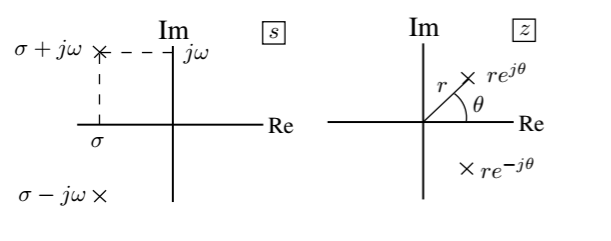
\includegraphics[width=0.9\linewidth]{Figuras/Ch05/fig1.PNG}}
\end{frame}

\begin{frame}{Relação entre os planos $s$ e $z$}
\centering

\scalebox{0.7}{\begin{tikzpicture}[scale=0.5]
			\draw (-4,-3) rectangle (4,3); %CLP
		\draw (-4,0) -- (-2.5,0); %Div in out
		\draw (-2.5,-3) -- (-2.5,3); %Div cartoes
		\draw (-1.5,-2.5) rectangle (0,2.5); %Mem dados
		\draw (0.5,-2.5) rectangle (3.5,-1); %Mem prog
		\draw (1,0) rectangle (3,2); %CPU
		\draw (-4,-5) rectangle (4,-3); %Alimentacao
		\draw (-2.5,4) rectangle (4,6); %Term de prog
		
		\draw (1,2.6) node {CLP};
		
		\draw (-3.25,1.5) node[text width=1.5cm,align=center,rotate=90] {\small Cartões de input};
		
		\draw (-3.25,-1.5) node[text width=1.5cm,align=center,rotate=90] {\small Cartões de output};
		
		\node at (2,1) {\small CPU};
		
		\node[rotate=90,text width=1.5cm,align=center] at (-0.75,0) {\small Memória de dados};
		
		\node[text width=2cm,align=center] at (2,-1.75) {\footnotesize Memória de programa};
		
		\node at (-6,0) {Campo};
		
		\node at (0,-4) {Alimentação};
		
		\node[text width=3cm,align=center] at (0.75,5) {Terminal de programação};
		
		\draw[-Latex] (-8,1.5) -- node[above] {Entradas} +(4,0);
		\draw[Latex-] (-8,-1.5) -- node[below] {Saídas} +(4,0);
		\draw[-Latex] (-2.5,1.5) -- +(1,0);
		\draw[Latex-] (-2.5,-1.5) -- +(1,0);
		\draw[-Latex] (0,1.5) -- +(1,0);
		\draw[Latex-] (0,0.5) -- +(1,0);
		\draw[Latex-] (2,0) -- +(0,-1);
		
		\draw[-Latex] (-1.5,4) -- +(0,-1);
		\draw[Latex-] (3,4) -- +(0,-1);
	\end{tikzpicture}}
\end{frame}


\begin{frame}{Relação entre os planos $s$ e $z$}
\begin{block}{Introdução}
A relação $ z=\text{e}^{sT} $ é a transformação entre a localização de polos no plano $s $ e a localização no plano $ z $.
A variável complexa $ s $ pode ser escrita como sendo $ s=\sigma+j\omega $. 

\vspace{0.5cm}

Logo, $ z=\text{e}^{(\sigma+j\omega)T} $, que pode ser escrito como \[ z=\underbrace{\text{e}^{\sigma T}}_{|z|}\underbrace{\text{e}^{j\omega T}}_{\phase{z}} \]
\end{block}
\end{frame}


\begin{frame}{Relação entre os planos $s$ e $z$ - Exemplo \#01}
\begin{block}{}
	\begin{align*}
		f(t)&=\text{e}^{-at}\, , \, t\geqslant 0& \quad \Rightarrow \quad F(s)&=\dfrac{1}{s+a}\\
		f(kT)&=\text{e}^{-akT}\, , \, k\geqslant 0& \quad \Rightarrow \quad F(z)&=\sum_{k=0}^{\infty} \text{e}^{-akT}\cdot z^{-k}=\sum_{k=0}^{\infty}\left( \dfrac{\text{e}^{-aT}}{z} \right)^{k}=\\
		& & &=\dfrac{1}{1-\dfrac{\text{e}^{-aT}}{z}}=\dfrac{z}{z-\text{e}^{-aT}}
	\end{align*}
	
	\begin{itemize}
		\item $ F(s) $ possui polo em $ s=-a $.
		\item $ F(z) $ possui polo em $ z=\text{e}^{-aT}=\text{e}^{sT} $, em que $ T\in \mathbb{R}_{>0} $ é o \textbf{período de amostragem.}
	\end{itemize}
\end{block}
\end{frame}


\begin{frame}{Relação entre os planos $s$ e $z$ - Exemplo \#01}
\begin{minipage}{0.45\linewidth}
	\centering
	
	\scalebox{0.45}{\newcommand{\innercolor}{gray!70!white}
	\newcommand{\outercolor}{gray!40!white}
	\newcommand{\leftcoil}{red!75!gray}
	\pgfmathsetmacro{\coilseparation}{0.02}
	
	\pgfmathsetmacro{\halflinewidth}{0.008}
	
	
	\begin{tikzpicture}[x={(\xx*1cm,\xy*1cm)},y={(\yx*1cm,\yy*1cm)},z={(\zx*1cm,\zy*1cm)}]
	\draw[\leftcoil, thick] (-0.02,5,1.125) -- +(0,2,0) (1.02,5,3.875) -- +(0,2,0);
	
	\draw[dashed,<->] ($ (-0.02,5,1.125)+(0,2,0) $) -- ($ (1.02,5,3.875)+(0,2,0) $);
	\node[rotate=85] at ($ (-0.02,5+2,1.125)!0.5!(1.02,5+2,3.875)+(0,0.2,0) $) {$ V_p $};
	
	\draw[-latex] (-0.02,6.5,1.325) -- node[above] {$ i_p $} +(0,-1,0);
	\draw[latex-] (1.02,0.02-0.5,1.3) -- node[above] {$ i_s $} +(0,-1,0);
	
	\filldraw[fill=\innercolor]  (0,1,1) -- (1,1,1) -- (1,4,1) -- (0,4,1) -- cycle;
	\filldraw[fill=\innercolor]  (1,4,1) -- (0,4,1) -- (0,4,4) -- (1,4,4) -- cycle;
	\filldraw[fill=\innercolor]  (0,0,0) -- (1,0,0) -- (1,0,5) -- (0,0,5) -- cycle;
	\filldraw[fill=\innercolor]  (0,0,5) -- (0,5,5) -- (1,5,5) -- (1,0,5) -- cycle;
	\filldraw[fill=\outercolor,even odd rule]    (0,0,0) -- (0,5,0) -- (0,5,5) -- (0,0,5) --cycle (0,1,1) -- (0,4,1) -- (0,4,4) -- (0,1,4) --cycle ;
	
	\begin{scope}
	\clip (0,3,1) -- (0,6,1) -- (0,6,4) -- (0,3,4);
	\foreach \z in {1.125,1.375,...,3.875}
	{   \draw[\leftcoil,thick] (0,5,\z) -- (-\coilseparation,5,\z) -- (-\coilseparation,4-\coilseparation,\z) -- (1+\coilseparation,4-\coilseparation,\z) -- (1+\coilseparation,4,\z);
	}
	\end{scope}
	
	
	\foreach \z in {1.25,1.75,...,3.75}
	{   \draw[blue,thick] (0,1,\z) -- (-\coilseparation,1,\z) -- (-\coilseparation,0-\coilseparation,\z) -- (1+\coilseparation,0-\coilseparation,\z) -- (1+\coilseparation,0,\z);
	}

	\draw[blue,thick] (1+\coilseparation,0+\coilseparation,1.1) -- +(0,-2,0) (-\coilseparation,1+\coilseparation,3.85) -- +(0,-3,0);
	
	\draw[dashed,<->] (1.02,-2+0.02,1.1) -- (-0.02,0.02-2,3.85);
	\node[rotate=-70] at ($ (1.02,-2+0.02,1.1)!0.5!(-0.02,0.02-2,3.85)+(0,-0.2,0) $) {$ V_s $};
	
	\draw[decorate,decoration={brace,amplitude=10pt},xshift=-4pt,yshift=0pt] (0,5,1.25) -- +(0,0,2.75);
	\draw[decorate,decoration={brace,amplitude=10pt},xshift=-4pt,yshift=0pt] (1.2,0,3.75) -- +(0,0,-2.6);
	\node[rotate=90] at (0,5.7,2.625) {$ N_p $ espiras};
	\node[rotate=-90] at (1.2,-0.5,2.5) {$ N_s $ espiras};
	
	\draw[dashed,postaction={decorate,decoration={markings,mark=between positions 0.1 and 1 step 0.2 with \arrow{Latex}}}] (0,4.5,0.5) -- (0,0.5,0.5) -- ++(0,0,4) -- ++(0,4,0) -- cycle;
	
	\draw[] (0,2.5,4.7)% -- +(0,-0.5,1.5)
	node[rotate=-10] {Fluxo magnético ($ \phi $)};
	
	\end{tikzpicture}}
\end{minipage}\tikzmark{p1}
\hfill
\begin{minipage}{0.45\linewidth}
	\centering
	
	\scalebox{0.45}{

\tikzset{every picture/.style={line width=0.75pt}} %set default line width to 0.75pt        

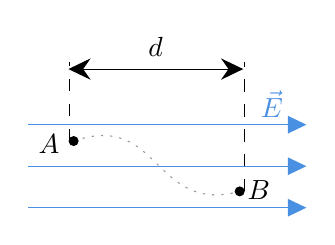
\begin{tikzpicture}[x=0.75pt,y=0.75pt,yscale=-1,xscale=1]
%uncomment if require: \path (0,300); %set diagram left start at 0, and has height of 300

%Curve Lines [id:da6177490068384819] 
\draw [color={rgb, 255:red, 155; green, 155; blue, 155 }  ,draw opacity=1 ] [dash pattern={on 0.84pt off 2.51pt}]  (137.88,127.88) .. controls (180,113.4) and (176,163.4) .. (217.88,152.13) ;


%Straight Lines [id:da7124330895115376] 
\draw [color={rgb, 255:red, 74; green, 144; blue, 226 }  ,draw opacity=1 ]   (116,120) -- (247,120) ;
\draw [shift={(250,120)}, rotate = 180] [fill={rgb, 255:red, 74; green, 144; blue, 226 }  ,fill opacity=1 ][line width=0.08]  [draw opacity=0] (8.93,-4.29) -- (0,0) -- (8.93,4.29) -- cycle    ;

%Straight Lines [id:da12792354611605283] 
\draw [color={rgb, 255:red, 74; green, 144; blue, 226 }  ,draw opacity=1 ]   (116,140) -- (247,140) ;
\draw [shift={(250,140)}, rotate = 180] [fill={rgb, 255:red, 74; green, 144; blue, 226 }  ,fill opacity=1 ][line width=0.08]  [draw opacity=0] (8.93,-4.29) -- (0,0) -- (8.93,4.29) -- cycle    ;

%Straight Lines [id:da4044562129660001] 
\draw [color={rgb, 255:red, 74; green, 144; blue, 226 }  ,draw opacity=1 ]   (116,160) -- (247,160) ;
\draw [shift={(250,160)}, rotate = 180] [fill={rgb, 255:red, 74; green, 144; blue, 226 }  ,fill opacity=1 ][line width=0.08]  [draw opacity=0] (8.93,-4.29) -- (0,0) -- (8.93,4.29) -- cycle    ;

%Shape: Circle [id:dp28224868607946574] 
\draw  [fill={rgb, 255:red, 0; green, 0; blue, 0 }  ,fill opacity=1 ] (135.75,127.88) .. controls (135.75,126.7) and (136.7,125.75) .. (137.88,125.75) .. controls (139.05,125.75) and (140,126.7) .. (140,127.88) .. controls (140,129.05) and (139.05,130) .. (137.88,130) .. controls (136.7,130) and (135.75,129.05) .. (135.75,127.88) -- cycle ;
%Shape: Circle [id:dp03942976292609046] 
\draw  [color={rgb, 255:red, 0; green, 0; blue, 0 }  ,draw opacity=1 ][fill={rgb, 255:red, 0; green, 0; blue, 0 }  ,fill opacity=1 ] (215.75,152.13) .. controls (215.75,150.95) and (216.7,150) .. (217.88,150) .. controls (219.05,150) and (220,150.95) .. (220,152.13) .. controls (220,153.3) and (219.05,154.25) .. (217.88,154.25) .. controls (216.7,154.25) and (215.75,153.3) .. (215.75,152.13) -- cycle ;
%Straight Lines [id:da5788684610773114] 
\draw  [dash pattern={on 4.5pt off 4.5pt}]  (135.75,127.88) -- (135.75,90) ;


%Straight Lines [id:da7063621547892809] 
\draw  [dash pattern={on 4.5pt off 4.5pt}]  (220,152.13) -- (220,90) ;


%Straight Lines [id:da8063380246624134] 
\draw    (138.35,93.2) -- (216.6,93.2) ;
\draw [shift={(219.6,93.2)}, rotate = 180] [fill={rgb, 255:red, 0; green, 0; blue, 0 }  ][line width=0.08]  [draw opacity=0] (10.72,-5.15) -- (0,0) -- (10.72,5.15) -- (7.12,0) -- cycle    ;
\draw [shift={(135.35,93.2)}, rotate = 0] [fill={rgb, 255:red, 0; green, 0; blue, 0 }  ][line width=0.08]  [draw opacity=0] (10.72,-5.15) -- (0,0) -- (10.72,5.15) -- (7.12,0) -- cycle    ;

% Text Node
\draw (233.4,110) node [color={rgb, 255:red, 74; green, 144; blue, 226 }  ,opacity=1 ]  {$\vec{E}$};
% Text Node
\draw (177.33,82.33) node   {$d$};
% Text Node
\draw (126,129.33) node   {$A$};
% Text Node
\draw (227.13,151.4) node   {$B$};


\end{tikzpicture}
}
\end{minipage}

\begin{block}{}
	\begin{itemize}
		\item Isso implica que todos os pontos no plano $ s $ tem seu \textbf{ponto correspondente} no plano $ z $.
	\end{itemize}
\end{block}

\begin{tikzpicture}[overlay, remember picture, scale=0.5]
	\draw (p1) ++(-2,0) node[above] {$ f(t) $} -- ++(1.5,0) node[circle, inner sep=1pt, draw, fill=black, name=p2] {} -- node[midway, name=p3] {} +(1.732, 1);
	\draw (p2) ++(1.732,0) node[circle, inner sep=1pt, fill=black, draw] {} -- +(1.5,0) node[above] {$ f(kT) $};
	\draw[->] ($ (p3)+(-0.2,0.4) $) node[above=-2pt, xshift=-2pt] {$ T $} to [out=330,in=100] +(0.4,-0.8);
\end{tikzpicture}
\end{frame}

\begin{frame}{Relação entre os planos $s$ e $z$}
\begin{block}{Observação}
\begin{itemize}
		\item A transformada de Laplace de um sinal amostrado pode ser dada por:
\end{itemize}
$$F^*(s) = \sum_{k=-\infty}^{\infty} f(kT) \text{e}^{-kTs}$$
\begin{itemize}
		\item Considerando um degrau unitário, por exemplo, temos que:
\end{itemize}
$$F^*(s) = \sum_{k=0}^{\infty} 1 \text{e}^{-kTs} = 1 + \text{e}^{-Ts} + \text{e}^{-2Ts} + \cdots = 1 + (\text{e}^{-Ts})^1 + (\text{e}^{-Ts})^2 + \cdots$$
\begin{itemize}
		\item Da série de potências sabemos que
\end{itemize}
$$1 + x + x^2 + \cdots = \dfrac{1}{1-x}, \ \text{se} \ |x| < 1$$
\end{block}
\end{frame}

\begin{frame}{Relação entre os planos $s$ e $z$}
\begin{block}{Observação}
\begin{itemize}
		\item Deste modo,
\end{itemize}
$$F^*(s) = \dfrac{1}{1 - \text{e}^{-Ts}}$$
\begin{itemize}
		\item O denominador de $F^*(s)$ não é um polinômio em $s$, mas são \textbf{funções transcendentais}. Uma consequência disso é que $F^*(s)$ tem \textbf{infinitos polos}.
		\item Além disso, $F^*(s)$ é uma \textbf{função periódica} em $s$, com período fundamental $j\omega_s$.
\end{itemize}
\end{block}
\end{frame}

\begin{frame}{Relação entre os planos $s$ e $z$}
\begin{block}{Mapeamento}
\begin{itemize}
	\item Considere o fato de que a maior frequência que pode ser representada é $\omega_s/2$.
	\item A \textbf{faixa primária} é dada por:
\end{itemize}
$$\Omega_p = \{ s = \sigma + j\omega \in \mathbb{C} \ | -\omega_s/2 \leq \omega \leq \omega_s/2 \} $$
\end{block}
\end{frame}

\begin{frame}{Relação entre os planos $s$ e $z$}
\centerline{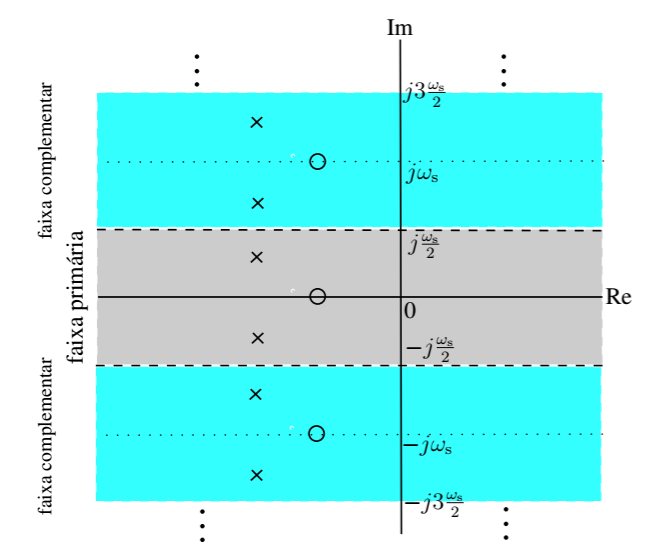
\includegraphics[width=0.75\linewidth]{Figuras/Ch05/fig4.PNG}}
\end{frame}

\begin{frame}{Relação entre os planos $s$ e $z$}
\begin{block}{Mapeamento}
\begin{itemize}
	\item Mapeamento da reta horizontal $s = \sigma + j\omega_s/2$
\end{itemize}
$$z = \text{e}^{sT} = \text{e}^{(\sigma + j\omega_s/2)T} = \text{e}^{\sigma T} \text{e}^{(j\omega_s/2) T} = -\text{e}^{\sigma T}$$
\begin{itemize}
	\item A reta horizontal $s$ no plano $s$ é mapeada para o eixo real negativo no plano $z$ ($\sigma \to -\infty \implies z \to 0^{-}$ e $\sigma \to \infty \implies z \to -\infty$).
\end{itemize}
\end{block}
\centerline{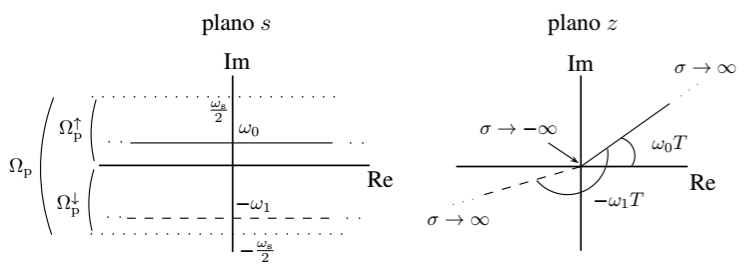
\includegraphics[width=0.9\linewidth]{Figuras/Ch05/fig2.PNG}}
\end{frame}

\begin{frame}{Relação entre os planos $s$ e $z$}
\begin{block}{Mapeamento}
\begin{itemize}
	\item Mapeamento da reta horizontal $s = \sigma - j\omega_s/2$
\end{itemize}
$$z = \text{e}^{sT} = \text{e}^{(\sigma - j\omega_s/2)T} = \text{e}^{\sigma T} \text{e}^{(-j\omega_s/2) T} = -\text{e}^{\sigma T}$$
\begin{itemize}
	\item A reta horizontal $s$ no plano $s$ é mapeada para o eixo real negativo no plano $z$ ($\sigma \to -\infty \implies z \to 0^{-}$ e $\sigma \to \infty \implies z \to -\infty$).
\end{itemize}
\end{block}
\centerline{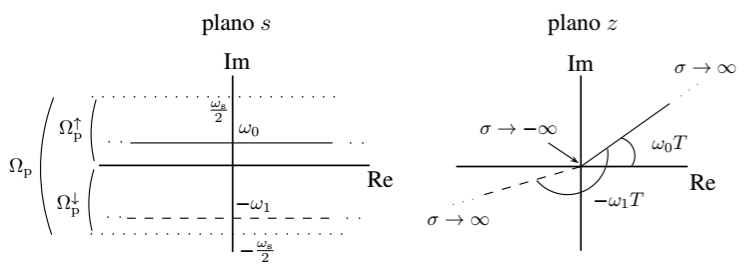
\includegraphics[width=0.9\linewidth]{Figuras/Ch05/fig2.PNG}}
\end{frame}

\begin{frame}{Relação entre os planos $s$ e $z$}
\begin{block}{Mapeamento}
\begin{itemize}
	\item Mapeamento da reta horizontal $s = \sigma + j\omega_0$
\end{itemize}
$$z = \text{e}^{sT} = \text{e}^{(\sigma + j\omega_0)T} = \text{e}^{\sigma T} \text{e}^{j\omega_0 T}$$
\begin{itemize}
	\item Semi-reta entre a origem do plano $z$ e $\infty$ (semi-plano superior).
	\item Ângulo $\omega_0 T$ com o eixo semi-real. 
\end{itemize}
\end{block}
\centerline{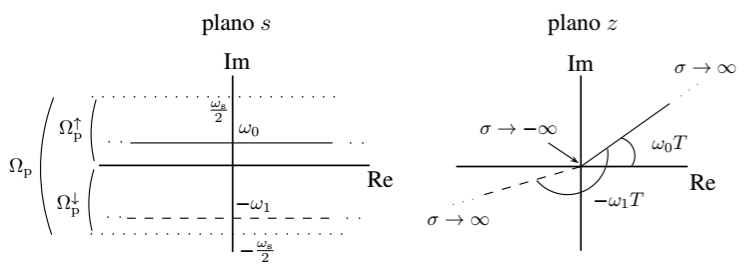
\includegraphics[width=0.9\linewidth]{Figuras/Ch05/fig2.PNG}}
\end{frame}

\begin{frame}{Relação entre os planos $s$ e $z$}
\begin{block}{Mapeamento}
\begin{itemize}
	\item Mapeamento da reta horizontal $s = \sigma - j\omega_1$
\end{itemize}
$$z = \text{e}^{sT} = \text{e}^{(\sigma - j\omega_1)T} = \text{e}^{\sigma T} \text{e}^{-j\omega_1 T}$$
\begin{itemize}
	\item Semi-reta entre a origem do plano $z$ e $-\infty$ (semi-plano inferior).
	\item Ângulo $\omega_1 T$ com o eixo semi-real. 
\end{itemize}
\end{block}
\centerline{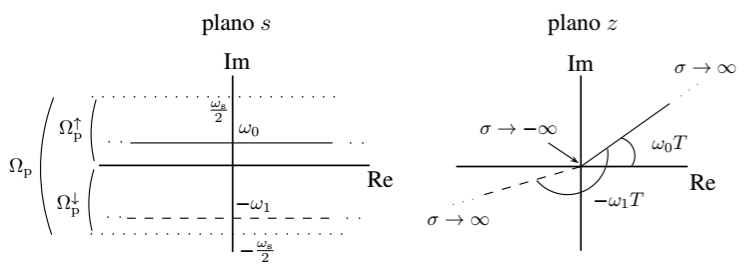
\includegraphics[width=0.9\linewidth]{Figuras/Ch05/fig2.PNG}}
\end{frame}

\begin{frame}{Região de estabilidade no plano $z$}
\begin{block}{Ponto A}
\begin{itemize}
	\item O ponto A (origem do plano $s$) é mapeado em:
\end{itemize}
$$z = \text{e}^{sT} = \text{e}^{0T} = 1$$
\end{block}
\centerline{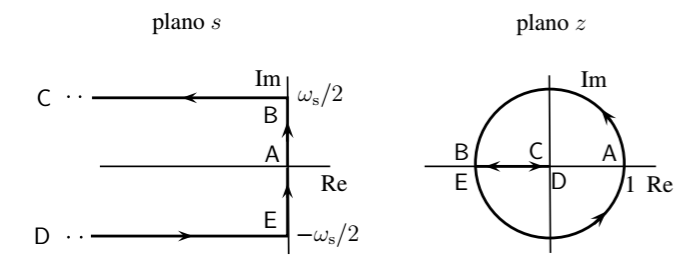
\includegraphics[width=0.9\linewidth]{Figuras/Ch05/fig3.PNG}}
\end{frame}

\begin{frame}{Região de estabilidade no plano $z$}
\begin{block}{Ponto A até ponto B}
\begin{itemize}
	\item Avançando a partir do ponto A em direção ao ponto B, temos que o mapeamento é:
\end{itemize}
$$z = \text{e}^{sT} = \text{e}^{(0+\omega)T} = \text{e}^{\omega T}, \quad 0 < \omega < \omega_s/2 \implies 0 < \theta < \pi$$
\end{block}
\centerline{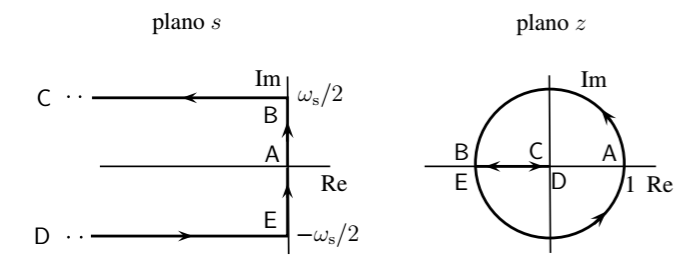
\includegraphics[width=0.9\linewidth]{Figuras/Ch05/fig3.PNG}}
\end{frame}

\begin{frame}{Região de estabilidade no plano $z$}
\begin{block}{Ponto B até ponto C}
\begin{itemize}
	\item Avançando a partir do ponto B em direção ao ponto C, temos que o mapeamento é dado no eixo real negativo do plano $z$ (\textit{conforme visto anteriormente}).
\end{itemize}
\end{block}
\centerline{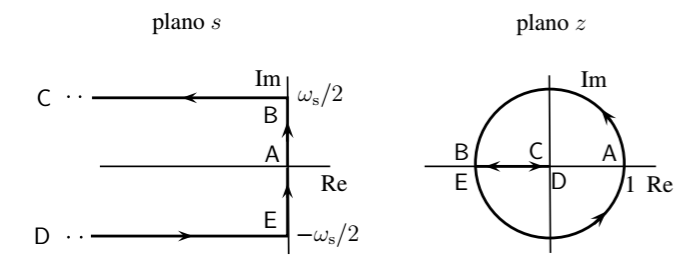
\includegraphics[width=0.9\linewidth]{Figuras/Ch05/fig3.PNG}}
\end{frame}

\begin{frame}{Região de estabilidade no plano $z$}
\begin{block}{Ponto C até ponto D}
\begin{itemize}
	\item Avançando a partir do ponto C em direção ao ponto D, temos que o mapeamento é:
\end{itemize}
$$\text{Ponto C:} \ z = \text{e}^{sT} = \text{e}^{(-\infty+\omega_s/2)T} = \text{e}^{-\infty T} \text{e}^{j\pi} = 0\phase{\pi}$$
$$\text{Ponto D:} \ z = \text{e}^{sT} = \text{e}^{(-\infty-\omega_s/2)T} = \text{e}^{-\infty T} \text{e}^{j-\pi} = 0\phase{-\pi}$$
\vspace{-0.3cm}
\begin{itemize}
    \item A mudança de fase indica uma mudança de direção.
\end{itemize}
\end{block}
\centerline{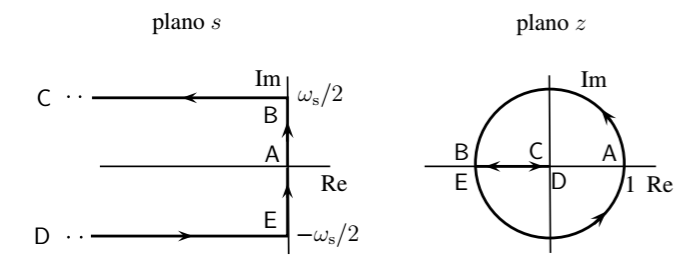
\includegraphics[width=0.8\linewidth]{Figuras/Ch05/fig3.PNG}}
\end{frame}

\begin{frame}{Região de estabilidade no plano $z$}
\begin{block}{Ponto D até ponto E}
\begin{itemize}
	\item Avançando a partir do ponto D em direção ao ponto E, temos que o mapeamento é dado no eixo real negativo do plano $z$ (\textit{conforme visto anteriormente}).
\end{itemize}
\end{block}
\centerline{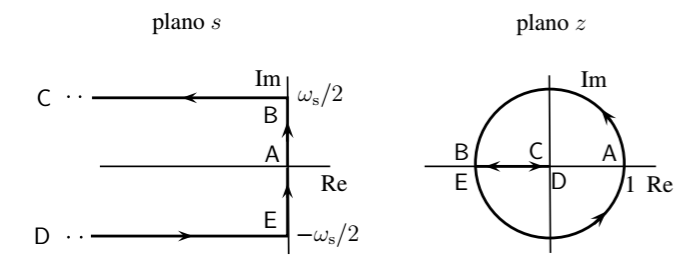
\includegraphics[width=0.9\linewidth]{Figuras/Ch05/fig3.PNG}}
\end{frame}

\begin{frame}{Região de estabilidade no plano $z$}
\begin{block}{Ponto E até ponto A}
\begin{itemize}
	\item Avançando a partir do ponto E em direção ao ponto A, temos que o mapeamento é:
\end{itemize}
$$z = \text{e}^{sT} = \text{e}^{(0+\omega)T} = \text{e}^{-\omega T}, \quad -\omega_s/2 < \omega < 0 \implies -\pi < \theta < 0$$
\end{block}
\centerline{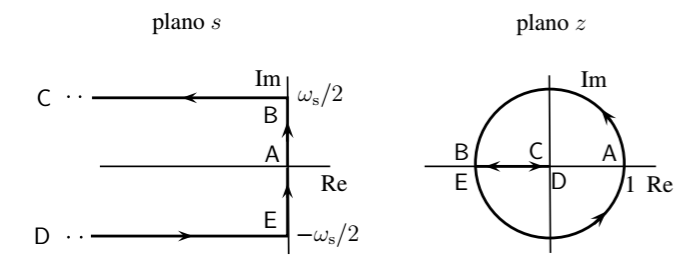
\includegraphics[width=0.9\linewidth]{Figuras/Ch05/fig3.PNG}}
\end{frame}

\begin{frame}{Região de estabilidade no plano $z$}
\begin{block}{Em resumo...}
\begin{itemize}
	\item O \textbf{eixo imaginário} do plano $ s $ é $ s=j\omega $, $ \sigma=0 $, e o lugar geométrico correspondente no plano $ z $ é:
	\[ \left. z=\text{e}^{\sigma T}\text{e}^{j\omega T} \quad \rightarrow \quad |z|=1 \text{ e }0<\phase{z} < \SI{360}{\degree}\right\rbrace \text{\textbf{círculo unitário.}}\]
	\item O \textbf{semiplano esquerdo} do plano $ s $ é dado por $ s=-\sigma+j\omega $, $ \sigma >0 $, e o lugar geométrico correspondente no plano $ z $ é:
	\[ \left. z=\text{e}^{\sigma T}\text{e}^{j\omega T} \quad \rightarrow \quad |z|=\text{e}^{-\sigma T}<1 \text{ e }\phase{z}= \omega T \right\rbrace \text{\textbf{dentro do círculo.}}  \]
	\item O \textbf{semiplano direito} do plano $ s $ é dado por $ s=\sigma+j\omega $, $ \sigma>0 $, e o lugar geométrico correspondente no plano $ z $ é:
	\[ \left. z=\text{e}^{\sigma T}\text{e}^{j\omega T} \quad \rightarrow \quad |z|=\text{e}^{\sigma T}>1 \text{ e }\phase{z}= \omega T \right\rbrace \text{\textbf{fora do círculo.}} \]
\end{itemize}
\end{block}
\end{frame}


\begin{frame}{Região de estabilidade no plano $z$}
\begin{minipage}{0.45\linewidth}
	\centering
	
	\scalebox{0.7}{

\tikzset{every picture/.style={line width=0.75pt}} %set default line width to 0.75pt        

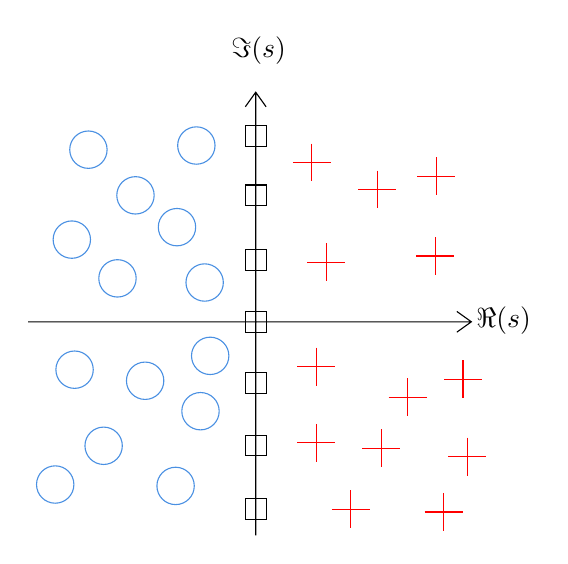
\begin{tikzpicture}[x=0.75pt,y=0.75pt,yscale=-1,xscale=1]
%uncomment if require: \path (0,300); %set diagram left start at 0, and has height of 300

%Shape: Axis 2D [id:dp27678030181731494] 
\draw  (40,160.6) -- (253.5,160.6)(149.6,50) -- (149.6,263.5) (246.5,155.6) -- (253.5,160.6) -- (246.5,165.6) (144.6,57) -- (149.6,50) -- (154.6,57)  ;
%Shape: Square [id:dp29640104318485094] 
\draw   (144.6,155.6) -- (154.6,155.6) -- (154.6,165.6) -- (144.6,165.6) -- cycle ;
%Shape: Square [id:dp5015049228757054] 
\draw   (144.6,125.7) -- (154.6,125.7) -- (154.6,135.7) -- (144.6,135.7) -- cycle ;
%Shape: Square [id:dp5724308304859749] 
\draw   (144.6,94.7) -- (154.6,94.7) -- (154.6,104.7) -- (144.6,104.7) -- cycle ;
%Shape: Square [id:dp8722658997981245] 
\draw   (144.6,66.2) -- (154.6,66.2) -- (154.6,76.2) -- (144.6,76.2) -- cycle ;
%Shape: Square [id:dp035501458242915174] 
\draw   (144.6,185.2) -- (154.6,185.2) -- (154.6,195.2) -- (144.6,195.2) -- cycle ;
%Shape: Square [id:dp23226558696093957] 
\draw   (144.6,215.2) -- (154.6,215.2) -- (154.6,225.2) -- (144.6,225.2) -- cycle ;
%Shape: Square [id:dp09667812864869552] 
\draw   (144.6,245.7) -- (154.6,245.7) -- (154.6,255.7) -- (144.6,255.7) -- cycle ;
\draw  [color={rgb, 255:red, 255; green, 0; blue, 0 }  ,draw opacity=1 ] (167.5,83.88) -- (185.75,83.88)(176.63,74.75) -- (176.63,93) ;
\draw  [color={rgb, 255:red, 255; green, 0; blue, 0 }  ,draw opacity=1 ] (199,96.88) -- (217.25,96.88)(208.13,87.75) -- (208.13,106) ;
\draw  [color={rgb, 255:red, 255; green, 0; blue, 0 }  ,draw opacity=1 ] (174.5,131.88) -- (192.75,131.88)(183.63,122.75) -- (183.63,141) ;
\draw  [color={rgb, 255:red, 255; green, 0; blue, 0 }  ,draw opacity=1 ] (227,128.88) -- (245.25,128.88)(236.13,119.75) -- (236.13,138) ;
\draw  [color={rgb, 255:red, 255; green, 0; blue, 0 }  ,draw opacity=1 ] (227.5,90.38) -- (245.75,90.38)(236.63,81.25) -- (236.63,99.5) ;
\draw  [color={rgb, 255:red, 255; green, 0; blue, 0 }  ,draw opacity=1 ] (169.67,182.21) -- (187.92,182.21)(178.79,173.08) -- (178.79,191.33) ;
\draw  [color={rgb, 255:red, 255; green, 0; blue, 0 }  ,draw opacity=1 ] (186.33,250.88) -- (204.58,250.88)(195.46,241.75) -- (195.46,260) ;
\draw  [color={rgb, 255:red, 255; green, 0; blue, 0 }  ,draw opacity=1 ] (231,252.21) -- (249.25,252.21)(240.13,243.08) -- (240.13,261.33) ;
\draw  [color={rgb, 255:red, 255; green, 0; blue, 0 }  ,draw opacity=1 ] (169.67,218.88) -- (187.92,218.88)(178.79,209.75) -- (178.79,228) ;
\draw  [color={rgb, 255:red, 255; green, 0; blue, 0 }  ,draw opacity=1 ] (242.33,225.54) -- (260.58,225.54)(251.46,216.42) -- (251.46,234.67) ;
\draw  [color={rgb, 255:red, 255; green, 0; blue, 0 }  ,draw opacity=1 ] (213.67,196.88) -- (231.92,196.88)(222.79,187.75) -- (222.79,206) ;
\draw  [color={rgb, 255:red, 255; green, 0; blue, 0 }  ,draw opacity=1 ] (240.33,188.21) -- (258.58,188.21)(249.46,179.08) -- (249.46,197.33) ;
\draw  [color={rgb, 255:red, 255; green, 0; blue, 0 }  ,draw opacity=1 ] (201,221.54) -- (219.25,221.54)(210.13,212.42) -- (210.13,230.67) ;
%Shape: Circle [id:dp01739200493370019] 
\draw  [color={rgb, 255:red, 74; green, 144; blue, 226 }  ,draw opacity=1 ] (60,77.67) .. controls (60,72.7) and (64.03,68.67) .. (69,68.67) .. controls (73.97,68.67) and (78,72.7) .. (78,77.67) .. controls (78,82.64) and (73.97,86.67) .. (69,86.67) .. controls (64.03,86.67) and (60,82.64) .. (60,77.67) -- cycle ;
%Shape: Circle [id:dp857755141402053] 
\draw  [color={rgb, 255:red, 74; green, 144; blue, 226 }  ,draw opacity=1 ] (82.67,99.67) .. controls (82.67,94.7) and (86.7,90.67) .. (91.67,90.67) .. controls (96.64,90.67) and (100.67,94.7) .. (100.67,99.67) .. controls (100.67,104.64) and (96.64,108.67) .. (91.67,108.67) .. controls (86.7,108.67) and (82.67,104.64) .. (82.67,99.67) -- cycle ;
%Shape: Circle [id:dp9246833060771249] 
\draw  [color={rgb, 255:red, 74; green, 144; blue, 226 }  ,draw opacity=1 ] (44,239) .. controls (44,234.03) and (48.03,230) .. (53,230) .. controls (57.97,230) and (62,234.03) .. (62,239) .. controls (62,243.97) and (57.97,248) .. (53,248) .. controls (48.03,248) and (44,243.97) .. (44,239) -- cycle ;
%Shape: Circle [id:dp8304441936419562] 
\draw  [color={rgb, 255:red, 74; green, 144; blue, 226 }  ,draw opacity=1 ] (118.67,177) .. controls (118.67,172.03) and (122.7,168) .. (127.67,168) .. controls (132.64,168) and (136.67,172.03) .. (136.67,177) .. controls (136.67,181.97) and (132.64,186) .. (127.67,186) .. controls (122.7,186) and (118.67,181.97) .. (118.67,177) -- cycle ;
%Shape: Circle [id:dp5059258663614863] 
\draw  [color={rgb, 255:red, 74; green, 144; blue, 226 }  ,draw opacity=1 ] (102.67,115) .. controls (102.67,110.03) and (106.7,106) .. (111.67,106) .. controls (116.64,106) and (120.67,110.03) .. (120.67,115) .. controls (120.67,119.97) and (116.64,124) .. (111.67,124) .. controls (106.7,124) and (102.67,119.97) .. (102.67,115) -- cycle ;
%Shape: Circle [id:dp21245040687156935] 
\draw  [color={rgb, 255:red, 74; green, 144; blue, 226 }  ,draw opacity=1 ] (52,121) .. controls (52,116.03) and (56.03,112) .. (61,112) .. controls (65.97,112) and (70,116.03) .. (70,121) .. controls (70,125.97) and (65.97,130) .. (61,130) .. controls (56.03,130) and (52,125.97) .. (52,121) -- cycle ;
%Shape: Circle [id:dp17429736806925722] 
\draw  [color={rgb, 255:red, 74; green, 144; blue, 226 }  ,draw opacity=1 ] (116,141.67) .. controls (116,136.7) and (120.03,132.67) .. (125,132.67) .. controls (129.97,132.67) and (134,136.7) .. (134,141.67) .. controls (134,146.64) and (129.97,150.67) .. (125,150.67) .. controls (120.03,150.67) and (116,146.64) .. (116,141.67) -- cycle ;
%Shape: Circle [id:dp33160849295458217] 
\draw  [color={rgb, 255:red, 74; green, 144; blue, 226 }  ,draw opacity=1 ] (74,139.67) .. controls (74,134.7) and (78.03,130.67) .. (83,130.67) .. controls (87.97,130.67) and (92,134.7) .. (92,139.67) .. controls (92,144.64) and (87.97,148.67) .. (83,148.67) .. controls (78.03,148.67) and (74,144.64) .. (74,139.67) -- cycle ;
%Shape: Circle [id:dp32709834546378724] 
\draw  [color={rgb, 255:red, 74; green, 144; blue, 226 }  ,draw opacity=1 ] (87.33,189) .. controls (87.33,184.03) and (91.36,180) .. (96.33,180) .. controls (101.3,180) and (105.33,184.03) .. (105.33,189) .. controls (105.33,193.97) and (101.3,198) .. (96.33,198) .. controls (91.36,198) and (87.33,193.97) .. (87.33,189) -- cycle ;
%Shape: Circle [id:dp8791724327388495] 
\draw  [color={rgb, 255:red, 74; green, 144; blue, 226 }  ,draw opacity=1 ] (53.33,183.67) .. controls (53.33,178.7) and (57.36,174.67) .. (62.33,174.67) .. controls (67.3,174.67) and (71.33,178.7) .. (71.33,183.67) .. controls (71.33,188.64) and (67.3,192.67) .. (62.33,192.67) .. controls (57.36,192.67) and (53.33,188.64) .. (53.33,183.67) -- cycle ;
%Shape: Circle [id:dp4794866171308949] 
\draw  [color={rgb, 255:red, 74; green, 144; blue, 226 }  ,draw opacity=1 ] (114,203.67) .. controls (114,198.7) and (118.03,194.67) .. (123,194.67) .. controls (127.97,194.67) and (132,198.7) .. (132,203.67) .. controls (132,208.64) and (127.97,212.67) .. (123,212.67) .. controls (118.03,212.67) and (114,208.64) .. (114,203.67) -- cycle ;
%Shape: Circle [id:dp5349657045143856] 
\draw  [color={rgb, 255:red, 74; green, 144; blue, 226 }  ,draw opacity=1 ] (67.33,220.33) .. controls (67.33,215.36) and (71.36,211.33) .. (76.33,211.33) .. controls (81.3,211.33) and (85.33,215.36) .. (85.33,220.33) .. controls (85.33,225.3) and (81.3,229.33) .. (76.33,229.33) .. controls (71.36,229.33) and (67.33,225.3) .. (67.33,220.33) -- cycle ;
%Shape: Circle [id:dp714149478603834] 
\draw  [color={rgb, 255:red, 74; green, 144; blue, 226 }  ,draw opacity=1 ] (102,239.67) .. controls (102,234.7) and (106.03,230.67) .. (111,230.67) .. controls (115.97,230.67) and (120,234.7) .. (120,239.67) .. controls (120,244.64) and (115.97,248.67) .. (111,248.67) .. controls (106.03,248.67) and (102,244.64) .. (102,239.67) -- cycle ;
%Shape: Circle [id:dp476022910470574] 
\draw  [color={rgb, 255:red, 74; green, 144; blue, 226 }  ,draw opacity=1 ] (112,75.67) .. controls (112,70.7) and (116.03,66.67) .. (121,66.67) .. controls (125.97,66.67) and (130,70.7) .. (130,75.67) .. controls (130,80.64) and (125.97,84.67) .. (121,84.67) .. controls (116.03,84.67) and (112,80.64) .. (112,75.67) -- cycle ;

% Text Node
\draw (151,30) node   {$\Im(s)$};
% Text Node
\draw (269,160) node   {$\Re(s)$};


\end{tikzpicture}}
\end{minipage}\tikzmark{p12}
\hfill
\begin{minipage}{0.45\linewidth}
	\centering
	
	\scalebox{0.7}{

\tikzset{every picture/.style={line width=0.75pt}} %set default line width to 0.75pt        

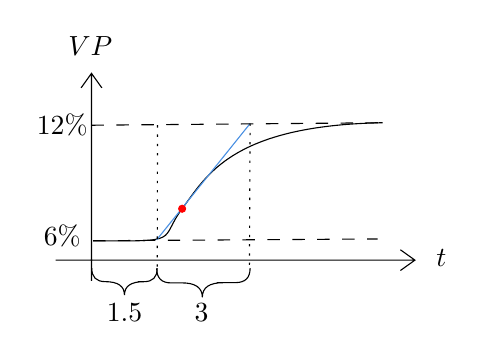
\begin{tikzpicture}[x=0.75pt,y=0.75pt,yscale=-1,xscale=1]
%uncomment if require: \path (0,300); %set diagram left start at 0, and has height of 300

%Shape: Axis 2D [id:dp8434144691544803] 
\draw  (61.27,196) -- (234.4,196)(78.58,106) -- (78.58,206) (227.4,191) -- (234.4,196) -- (227.4,201) (73.58,113) -- (78.58,106) -- (83.58,113)  ;
%Curve Lines [id:da3393494842698659] 
\draw    (79.33,186.67) .. controls (123.2,187) and (110.65,186.84) .. (122.25,171.24) .. controls (133.85,155.64) and (145.88,131.07) .. (218.8,129.8) ;


%Straight Lines [id:da773558557641419] 
\draw [color={rgb, 255:red, 74; green, 144; blue, 226 }  ,draw opacity=1 ]   (155,130.2) -- (110,186.2) ;


%Shape: Circle [id:dp28048312241562945] 
\draw  [color={rgb, 255:red, 255; green, 0; blue, 0 }  ,draw opacity=1 ][fill={rgb, 255:red, 255; green, 0; blue, 0 }  ,fill opacity=1 ] (120.58,171.24) .. controls (120.58,170.32) and (121.33,169.57) .. (122.25,169.57) .. controls (123.17,169.57) and (123.92,170.32) .. (123.92,171.24) .. controls (123.92,172.16) and (123.17,172.91) .. (122.25,172.91) .. controls (121.33,172.91) and (120.58,172.16) .. (120.58,171.24) -- cycle ;
%Straight Lines [id:da6828905031101673] 
\draw  [dash pattern={on 4.5pt off 4.5pt}]  (78.6,131) -- (218.8,129.8) ;


%Straight Lines [id:da012395283086218845] 
\draw  [dash pattern={on 4.5pt off 4.5pt}]  (79.33,186.67) -- (216.4,185.8) ;


%Shape: Brace [id:dp15969553307240192] 
\draw   (78.71,199.86) .. controls (78.7,204.19) and (80.87,206.35) .. (85.2,206.36) -- (85.2,206.36) .. controls (91.38,206.37) and (94.47,208.54) .. (94.46,212.87) .. controls (94.47,208.54) and (97.56,206.38) .. (103.75,206.39)(100.96,206.38) -- (103.75,206.39) .. controls (108.08,206.4) and (110.24,204.24) .. (110.25,199.91) ;
%Shape: Brace [id:dp058145123409859556] 
\draw   (110,200) .. controls (110.02,204.67) and (112.36,206.99) .. (117.03,206.97) -- (121.96,206.95) .. controls (128.63,206.92) and (131.97,209.23) .. (131.99,213.9) .. controls (131.97,209.23) and (135.29,206.89) .. (141.96,206.86)(138.96,206.87) -- (148.03,206.83) .. controls (152.7,206.81) and (155.02,204.47) .. (155,199.8) ;
%Straight Lines [id:da9569907625895342] 
\draw  [dash pattern={on 0.84pt off 2.51pt}]  (155,130.2) -- (154.68,198.45) ;


%Straight Lines [id:da25982411660347404] 
\draw  [dash pattern={on 0.84pt off 2.51pt}]  (110.4,131) -- (110.25,200.52) ;



% Text Node
\draw (247.2,194.8) node   {$t$};
% Text Node
\draw (78,93) node   {$VP$};
% Text Node
\draw (94.53,221.43) node   {$\SI{1.5}{\second}$};
% Text Node
\draw (131.58,221.2) node   {$\SI{3}{\second}$};
% Text Node
\draw (64.5,131) node   {$12\%$};
% Text Node
\draw (64.5,184.5) node   {$6\%$};


\end{tikzpicture}
}
\end{minipage}

\begin{block}{Conclusão}
	\textbf{Um sistema causal será estável se todos os polos em malha fechada da função de transferência em $ \bm{z} $ estiverem dentro do círculo unitário do plano $ \bm{z} $.}
\end{block}

\begin{tikzpicture}[overlay, remember picture, scale=0.5]
\draw[->] ($ (p12)+(0,0) $) node[above=5pt, xshift=15pt] {$ z=\text{e}^{sT} $} to [out=45,in=135] +(2,0);
\end{tikzpicture}
\end{frame}


\begin{frame}{Relação entre os planos $s$ e $z$}
\begin{block}{Importante}
Importante observar que o mapeamento exponencial, na prática, é pouco realizado, por limitação das técnicas digitais e que por causa disso é realizado por meio de \textbf{aproximações}, como veremos nas próximas aulas.
\end{block}
\end{frame}


\begin{frame}{Relação entre os planos $s$ e $z$}
\begin{block}{Observação}
\begin{itemize}
	\item Valores constantes de $ \sigma $ são mapeados em um círculo dentro do círculo unitário no plano $ z $.
	\item Grandes valores de $ \sigma $ representam pequenos valores de constante de tempo, logo um decaimento ou crescimento mais veloz.
\end{itemize}
\end{block}

%\vspace{0.5cm}

\begin{minipage}{0.45\linewidth}
	\centering
	
	\scalebox{0.9}{\begin{tikzpicture}
	\draw[->] (-2.5,0) -- (2.5,0) node[right] {$ \sigma $};
	\draw[->] (0,-2) -- (0,2) node[above] {$ j\omega $};
	
	\draw (0,0) node[below left] {$ 0 $};
	
	\draw (-1,-2) -- (-1,2) (1,-2) -- (1,2);
	
	\node [above left] at (-1,0) {$ -\sigma_1 $};
	\node [above right] at (1,0) {$ \sigma_2 $};
\end{tikzpicture}}
\end{minipage}\tikzmark{p13}
\hfill
\begin{minipage}{0.45\linewidth}
	\centering
	
	\scalebox{0.65}{

\tikzset{every picture/.style={line width=0.75pt}} %set default line width to 0.75pt        

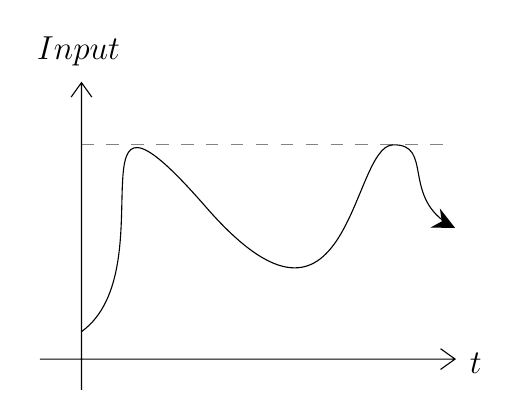
\begin{tikzpicture}[x=0.75pt,y=0.75pt,yscale=-1,xscale=1]
%uncomment if require: \path (0,300); %set diagram left start at 0, and has height of 300

%Straight Lines [id:da26643584263795916] 
\draw [color={rgb, 255:red, 131; green, 131; blue, 131 }  ,draw opacity=1 ] [dash pattern={on 4.5pt off 4.5pt}]  (90,100) -- (270,100) ;


%Shape: Axis 2D [id:dp7046941980103143] 
\draw  (70,203.2) -- (270,203.2)(90,70) -- (90,218) (263,198.2) -- (270,203.2) -- (263,208.2) (85,77) -- (90,70) -- (95,77)  ;
%Curve Lines [id:da03413665677920852] 
\draw    (90,190) .. controls (132.33,159.33) and (80.33,50) .. (150,130) .. controls (219.67,210) and (219.67,100.67) .. (240,100) .. controls (259.93,99.35) and (243.68,125.58) .. (268.43,139.18) ;
\draw [shift={(270,140)}, rotate = 206.28] [fill={rgb, 255:red, 0; green, 0; blue, 0 }  ][line width=0.75]  [draw opacity=0] (10.72,-5.15) -- (0,0) -- (10.72,5.15) -- (7.12,0) -- cycle    ;


% Text Node
\draw (88.5,55) node   {\large $Input$};
% Text Node
\draw (280,205) node   {\large $t$};


\end{tikzpicture}
}
\end{minipage}

\begin{tikzpicture}[overlay, remember picture, scale=0.5]
\draw[-Implies, double distance=2pt] ($ (p13)+(0.5,1) $) -- +(1,0);
\end{tikzpicture}
\end{frame}


\begin{frame}{Relação entre os planos $s$ e $z$}
\begin{block}{Observação}
\begin{itemize}
	\item Valores constantes de $\omega$ são mapeados de forma radial no plano $ z $.
\end{itemize}
\end{block}

\vspace{0.5cm}

\begin{minipage}{0.45\linewidth}
	\centering
	
	\scalebox{1}{

\tikzset{every picture/.style={line width=0.75pt}} %set default line width to 0.75pt        

\begin{tikzpicture}[x=0.75pt,y=0.75pt,yscale=-1,xscale=1]
%uncomment if require: \path (0,300); %set diagram left start at 0, and has height of 300

%Straight Lines [id:da45173516768188793] 
\draw [color={rgb, 255:red, 131; green, 131; blue, 131 }  ,draw opacity=1 ] [dash pattern={on 4.5pt off 4.5pt}]  (110,131.33) -- (290,131.33) ;


%Shape: Axis 2D [id:dp17702348361548204] 
\draw  (90,223.2) -- (290,223.2)(110,90) -- (110,238) (283,218.2) -- (290,223.2) -- (283,228.2) (105,97) -- (110,90) -- (115,97)  ;
%Curve Lines [id:da6473783232781454] 
\draw    (110.42,151.33) .. controls (152.75,120.66) and (159.67,124.33) .. (151,174.99) .. controls (142.33,225.66) and (200,152.99) .. (220.33,152.33) .. controls (240.26,151.67) and (268.19,192.64) .. (294.71,206.83) ;
\draw [shift={(296.33,207.66)}, rotate = 206.28] [fill={rgb, 255:red, 0; green, 0; blue, 0 }  ][line width=0.75]  [draw opacity=0] (10.72,-5.15) -- (0,0) -- (10.72,5.15) -- (7.12,0) -- cycle    ;


% Text Node
\draw (108.5,75) node   {\large $Output$};
% Text Node
\draw (300,225) node   {\large $t$};


\end{tikzpicture}
}
\end{minipage}\tikzmark{p14}
\hfill
\begin{minipage}{0.45\linewidth}
	\centering
	
	\scalebox{0.7}{\begin{tikzpicture}[scale=1.5]
	\draw[-latex] (-1.5,0) -- (2,0) node[right] {$ \Re(z) $};
	\draw[-latex] (0,-1.5) -- (0,1.5) node[above] {$ \Im(z) $};
	
	\draw[dashed] (0,0) circle (1);
	
	\node [above right,rotate=45] at ($ (0.3,0)+(1.8pt,-1.5pt) $) {\footnotesize $ \theta=\omega_1T $};
	
	\draw[->] (0,0) -- (150:1) node[left] {$ r=1 $};
	
	\draw[-latex] (0,0) -- (45:1cm);
	\draw[-latex] (0,0) -- (45:1.5cm);
	\draw (0,0) -- (45:1.7cm);
	
	\draw[-stealth] (0.3,0) arc (0:45:0.3);
	
	\draw (0,0) node[below left] {$ 0 $};
\end{tikzpicture}}
\end{minipage}

\begin{tikzpicture}[overlay, remember picture, scale=0.5]
\draw[-Implies, double distance=2pt] ($ (p14)+(0.5,1) $) node[name=p24] {} -- +(1,0);
\node[below=1cm of p24, align=center] {
	$ \begin{aligned}
	z=\text{e}^{sT}&=\text{e}^{\sigma T}\text{e}^{j\omega T}\\
				   &=r\phase{\theta}
	\end{aligned} $
};
\end{tikzpicture}
\end{frame}

\begin{frame}{O plano $w$}
\begin{block}{Introdução}
\begin{itemize}
    \item Conforme vimos anteriormente, a transformada de Laplace de um sinal amostrado introduz um número infinito de polos (já que temos a presença do termo $\text{e}^{sT}$).
    \item Ao mapearmos para o plano $z$ (onde $z = \text{e}^{sT}$) este problema é contornado.
    \item Além disso, o \textbf{limite de estabilidade} deixa de ser o eixo imaginário (plano $s$) e passa a ser a circunferência de raio unitário (plano $z$). 
\end{itemize}
\end{block}
\end{frame}

\begin{frame}{O plano $w$}
\begin{block}{Contextualização}
\begin{itemize}
    \item Em algumas aplicações (como, por exemplo, analisar a estabilidade de sistemas usando o critério de estabilidade de Routh-Hurwitz -- \textit{veja o capítulo 7}) pode ser interessante voltar a mapear o limite de estabilidade para o \textbf{eixo imaginário}, porém \textbf{sem recorrer ao uso de funções transcendentais}, para não incorrer  no problema de ter infinitos polos.
    \item Deste modo, se
\end{itemize}
$$z = \text{e}^{sT} \implies s = \dfrac{1}{T} \text{ln} \, z$$
\begin{itemize}
   \item[] está descartado o seu uso, por se tratar de uma função transcendental.
\end{itemize}
\end{block}
\end{frame}

\begin{frame}{Relação entre os planos $z$ e $w$}
\begin{block}{Definição}
\begin{itemize}
    \item A expansão em séries de potências nos diz que:
\end{itemize}
$$\text{ln} \, z = 2 \sum_{k=0}^{\infty} \dfrac{1}{2k+1} \left(\dfrac{z-1}{z+1}\right)^{2k+1}$$
\begin{itemize}
    \item Truncando depois do primeiro termo, temos que:
\end{itemize}
$$\text{ln} \, z \approx 2 \left(\dfrac{z-1}{z+1}\right)$$
\begin{itemize}
    \item Deste modo, como $s = \dfrac{1}{T} \text{ln} \, z$, temos que:
\end{itemize}
$$\boxed{w = \dfrac{2}{T} \left(\dfrac{z-1}{z+1}\right)}$$
\end{block}
\end{frame}

\begin{frame}{Relação entre os planos $z$ e $w$}
\begin{block}{Definição}
\begin{itemize}
    \item O inverso também é válido. Logo:
\end{itemize}
$$\boxed{z = \dfrac{1+(T/2)w}{1-(T/2)w}}$$
\end{block}
\end{frame}

\frame{
\frametitle{Exercícios}
\begin{block}{}
01. Mostre que o eixo real do plano $s$, ou seja, $s = \sigma$, $\forall \sigma$ é mapeado por $z = \text{e}^{sT}$ para o semi-eixo real positivo no plano $z$. 
\end{block}
}

\frame{
\frametitle{Referências e exercícios complementares}
\begin{itemize}
\item AGUIRRE, Luis A. Controle de Sistemas Amostrados, 1 ed. [s.n.], 2019.
\end{itemize}
\centering{\alert{Página 96 - \textbf{Capítulo 3}}} \\
}


